\documentclass[
    NAME={Dr. Helga Ingimundardóttir},
    EMAIL={helgaingim@hi.is},
    FACULTY={Industrial Engineering},
    SUBTITLE={From Smart Algorithms in Fish Portioning to Pioneering Pipelines in Long-Range DNA Sequencing and Digital Travel},
    SEMINAR={IVT Faculty Gathering},
    DATE={September 6, 2023}
]{hi-latex/hi-beamer}
\title{Databases, DNA \& Digital Detours}

\usepackage[style=authoryear,backend=bibtex]{biblatex}
\addbibresource{references.bib} % replace with the name of your .bib file

\begin{document}

\begin{frame}{Agenda}
\tableofcontents
\end{frame}

\section{Personal Introduction}

\begin{frame}{My Journey: From Math to Academia}
\emph{Academic Evolution:}
\begin{itemize}
    \item Started with math; transitioned to comp. science and applied math.
    \item Master's in Computational Engineering cemented my direction.
\end{itemize}

\emph{Into the Academic Realm:}
\begin{itemize}
    \item Began as TPR's TA, grew into PhD and \textit{much} later, Post-Doc roles.
    \item Returned to teaching after a decade; found confidence in maturity.
\end{itemize}

\emph{Merging Industry \& Academia:}
\begin{itemize}
    \item Tapped into industry insights: software dev., AI, and data science.
\end{itemize}

\emph{Passions Beyond Academia}:
\begin{itemize}
    \item Textile enthusiast: garment sewing, knitting, lace making, machine embroidery.
    \item A recent aficionado of modern board games.
\end{itemize}
\end{frame}

\section{Academic Background}
\begin{frame}{Educational Journey}
\begin{itemize}
    \item \emph{B.Sc. in Mathematics} (Emphasis on Computer Science), University of Iceland, 2005-2008.
    \item \emph{M.Sc. in Computational Engineering}, University of Iceland, 2008-2010:
    \begin{itemize}
        \item Erasmus exchange at Université de Valenciennes.
        \item Focus: fouling in cross-flow heat exchangers with Prof. Sylvain Lalot
    \end{itemize}
    \item \emph{Ph.D. in Computational Engineering}, University of Iceland:
    \begin{itemize}
        \item PhD Stipend from autumn 2009-2012
        \item Started working full-time at Valka Jan 2013, PhD in spare time.
        \item Defended in June 2016
    \end{itemize}
    \item \emph{Diploma in Teaching Studies for Higher Education}, 2010-2012.
    \begin{itemize}
        \item Taught Operations Research 2011 and 2012
    \end{itemize}
\end{itemize}
\end{frame}


\section{Research Highlights}
\begin{frame}{Dissertation}
\begin{itemize}
    \item Case Study on supervised learning approaches in dispatching rules for \emph{Job Shop Scheduling Problem} (JSSP).
    \item Introduction of \emph{Analysis \& Learning Iterative Consecutive Executions} (ALICE) framework for effective training.
    \item Emphasized Training Data:
    \begin{itemize}
        \item Should match the induced data distribution via active imitation learning.
        \item Labels are derived using an expert policy.
        \item Account for data balance with respect to dispatching step.
        \item Use of $(K-k)$ roll-outs to augment stepwise features.
    \end{itemize}
    \item Expert policy not just for labeling; also reveals vulnerabilities in the scheduling process.
    \item While stepwise optimality often aligns with good end performance, there's room for understanding trajectory deviations.
    \item Approach leverages preference learning but is flexible for substitutions and other scheduling problems.
\end{itemize}
\end{frame}

\begin{frame}{Selected Publications \& Contributions}

    \emph{Ph.D. Research}
     {\scriptsize\begin{itemize}
        \item \fullcite{isda11}
        \item \fullcite{Ingimundardottir2018}
        \item \fullcite{InRu15a} (Nominated for Best Paper Award at LION 2015)
    \end{itemize}}

    \emph{Master's Research}
    {\scriptsize\begin{itemize}
    \item \fullcite{fouling}
    \item \fullcite{fouling}
    \end{itemize}}

    \emph{deCODE genetics Research}
    {\scriptsize\begin{itemize}
        \item \fullcite{decodeBeyter}
        \item \fullcite{Holley2021}
    \end{itemize}}
\end{frame}

\section{Professional Experiences}
\begin{frame}{Real-world Engagements and Contributions}
\begin{itemize}
    \item \emph{deCODE genetics} (2016-2021):
    \begin{itemize}
        \item Designed and managed the \emph{ONT} long-range sequencing analysis pipeline.
        \item Key role in handling 6 petabytes of data.
        \item Contributed to significant research projects.
    \end{itemize}

    \item \emph{Valka} (2013-2015):
    \begin{itemize}
        \item Developed fish bone detection algorithms.
        \item Implemented fish portioning algorithms for multiple species.
    \end{itemize}

    \item \emph{AGR Dynamics}: SQL consultant for supply chain management system, AGR 5.

    \item \emph{CCP Games}: Developed near-realtime recommendation engine for new EVE Online players.

    \item \emph{Travelshift} (Head of AI Research): Led AI consultancy team optimizing travel plans on \href{https://guidetoeurope.com/best-vacation-packages}{GuideToEurope.com}.

    \item Advisor for \emph{RANNÍS} Technology Development Fund 2015 \& 2023.
\end{itemize}
\end{frame}

\section{Teaching Philosophy}
\begin{frame}{Teaching Focus}
    \begin{itemize}
        \item \emph{Real-World Relevance:} Connecting classroom lessons with real-world applications,
        emphasizing the power of teamwork in solving modern challenges.

        \item \emph{Technical Writing:} Emphasizing the importance of clear, concise communication.
        Teaching students the art of turning data and results into compelling narratives.

        \item \emph{Data Storytelling:} Equipping students with tools and techniques for effective data visualization.
        Encouraging the creation of visual narratives from raw data.

        \item \emph{Open Collaboration with GitHub:}
            \begin{itemize}
                \item Highlighting GitHub as an essential workforce skill.
                \item Using it for team assignments, fostering practical hands-on experience.
            \end{itemize}

    \end{itemize}
\end{frame}


\section{Looking Ahead}
\begin{frame}{Now \& Future Work}
\emph{Current Endeavors}:
    \begin{itemize}
        \item Active contribution to \emph{IDeLM}.
        \item Collaborative work with TPR on fairness model for \emph{Anesthetist's Peel Assignment Problem}.
    \end{itemize}
    \bigskip
\emph{Future Aspirations}:
        \begin{itemize}
            \item Carve a niche at the crossroads of AI and creativity.
            \item Dive into garment pattern optimization using 2D free-form binpacking.
            \item Utilize generative AI for an innovative knitting program.
        \end{itemize}
\end{frame}

\begin{frame}{Get In Touch}
Always open for collaboration, brainstorming, and discussions.

\bigskip

\begin{itemize}
        \item \emph{E-mail}: \href{mailto:helgaingim@hi.is}{helgaingim@hi.is}
        \item \emph{Temporary Office}: Squatting in TPR's office. Feel free to drop by for discussions!
    \end{itemize}
\end{frame}

\begin{frame}{Upcoming Talk: Save the Date!}
\begin{tikzpicture}[remember picture,overlay]
    \node[anchor=north west, inner sep=0pt, opacity=0.3] at (current page.north west)
        {
\includegraphics[width=\paperwidth, height=\paperheight]{iskisur-background.jpg}};
\end{tikzpicture}
\begin{columns}
    \begin{column}{0.65\textwidth}
    \emph{Haustráðstefna Advania}\\
    \emph{Date:} 8th September 2023\\
    \emph{Time:} 14:15 - 14:30\\
    \emph{Venue:} Harpa / Online\\
    \bigskip
    \begin{alertblock}{Pushing Boundaries: A Data-Driven Dive into \emph{Legend of the Ice People}}
    Unravel the unexpected synergy of literature and data science as we navigate the narrative maze of Margit Sandemo's
    cherished series, extracting insights from its many incarnations -- from print to audio to podcasts, showcasing the
    transformative power of data in unexpected territories.
    \end{alertblock}
\end{column}
\begin{column}{0.35\textwidth}
    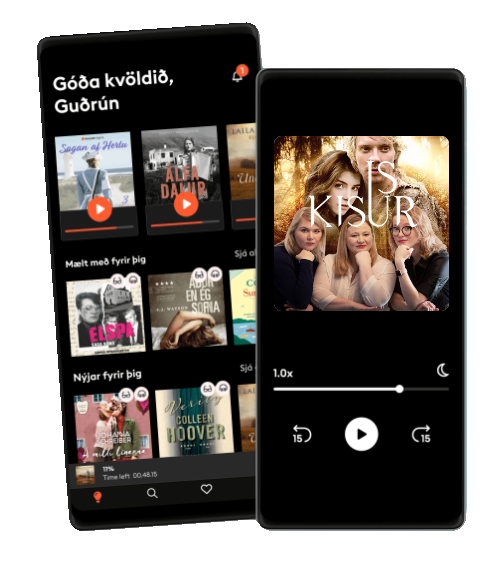
\includegraphics[width=\textwidth]{iskisur.jpg}
\end{column}
\end{columns}

\end{frame}


\end{document}
